\section{Aim}
The aim of this experiment is to study the working principle of a diode laser proposing a spectroscopy of rubidium using an optical grating.


\section{Theoretical Foundations}
\subsection{Basics of Lasers}

\noindent
A laser (light amplification by stimulated emission of radiation) is a source of intensive coherent light through photon emission.
Therefore a laser can be used to excite atoms and to pump energy into a medium.
In atoms the electrons possess different discrete energy levels.
The basic priciples of photon electron interaction are shown in figure (),
that includes absorption, spontaneous and stimulated emission of a photon.


%\begin{figure}
%  \centering
%  \includegraphics[width=9cm]{zustand.pdf}
%  \caption{Aufbau einer Röntgenröhre} %\cite{V603}}
%  \label{fig:zustand}
%\end{figure}

\noindent
If a photon $\gamma$ has enough energy to excite an electron from a lower to a higher state, it can be absorbed.
Spontaneous emission discribes the opposite, where a photon is emitted due to a transition to a lower energy level that happens spontaneously.
The  most interesting process when it comes to a laser system, is the stimulated emission.
Stimulated emission is induced by an incoming photon which energy has to be equal to the gap energy.
As a result two coherent photons with the same direction and energy will be emitted, what is fundamental to run a laser.
In order to reach a higher probability of stimulated emission a population inversion is needed, where the electron density in the higher state has to be higher than in the lower state.
This can only be achieved through pumping in an at least three energy level system as shown in figure ().

%\begin{figure}
%  \centering
%  \includegraphics[width=9cm]{zustand.pdf}
%  \caption{Aufbau einer Röntgenröhre} %\cite{V603}}
%  \label{fig:zustand}
%\end{figure}

\noindent
The transition from level 1 to level 3 is induced by absorption of energy through continuously pumping with electric current.
Electrons in level 3 are spontaneously relaxing in a lower state 2 with a high decay rate.
Considering that level 3 has a higher decay rate than level 2 the pumping creates the required population inversion between level 2 and level 1.


\subsection{Diode-Laser}
\noindent
A lasing system is in need of four essential components.
In the following the components itself and their net gain shown in figure \ref{fig:netgain} will be discussed.

\begin{figure}
  \centering
  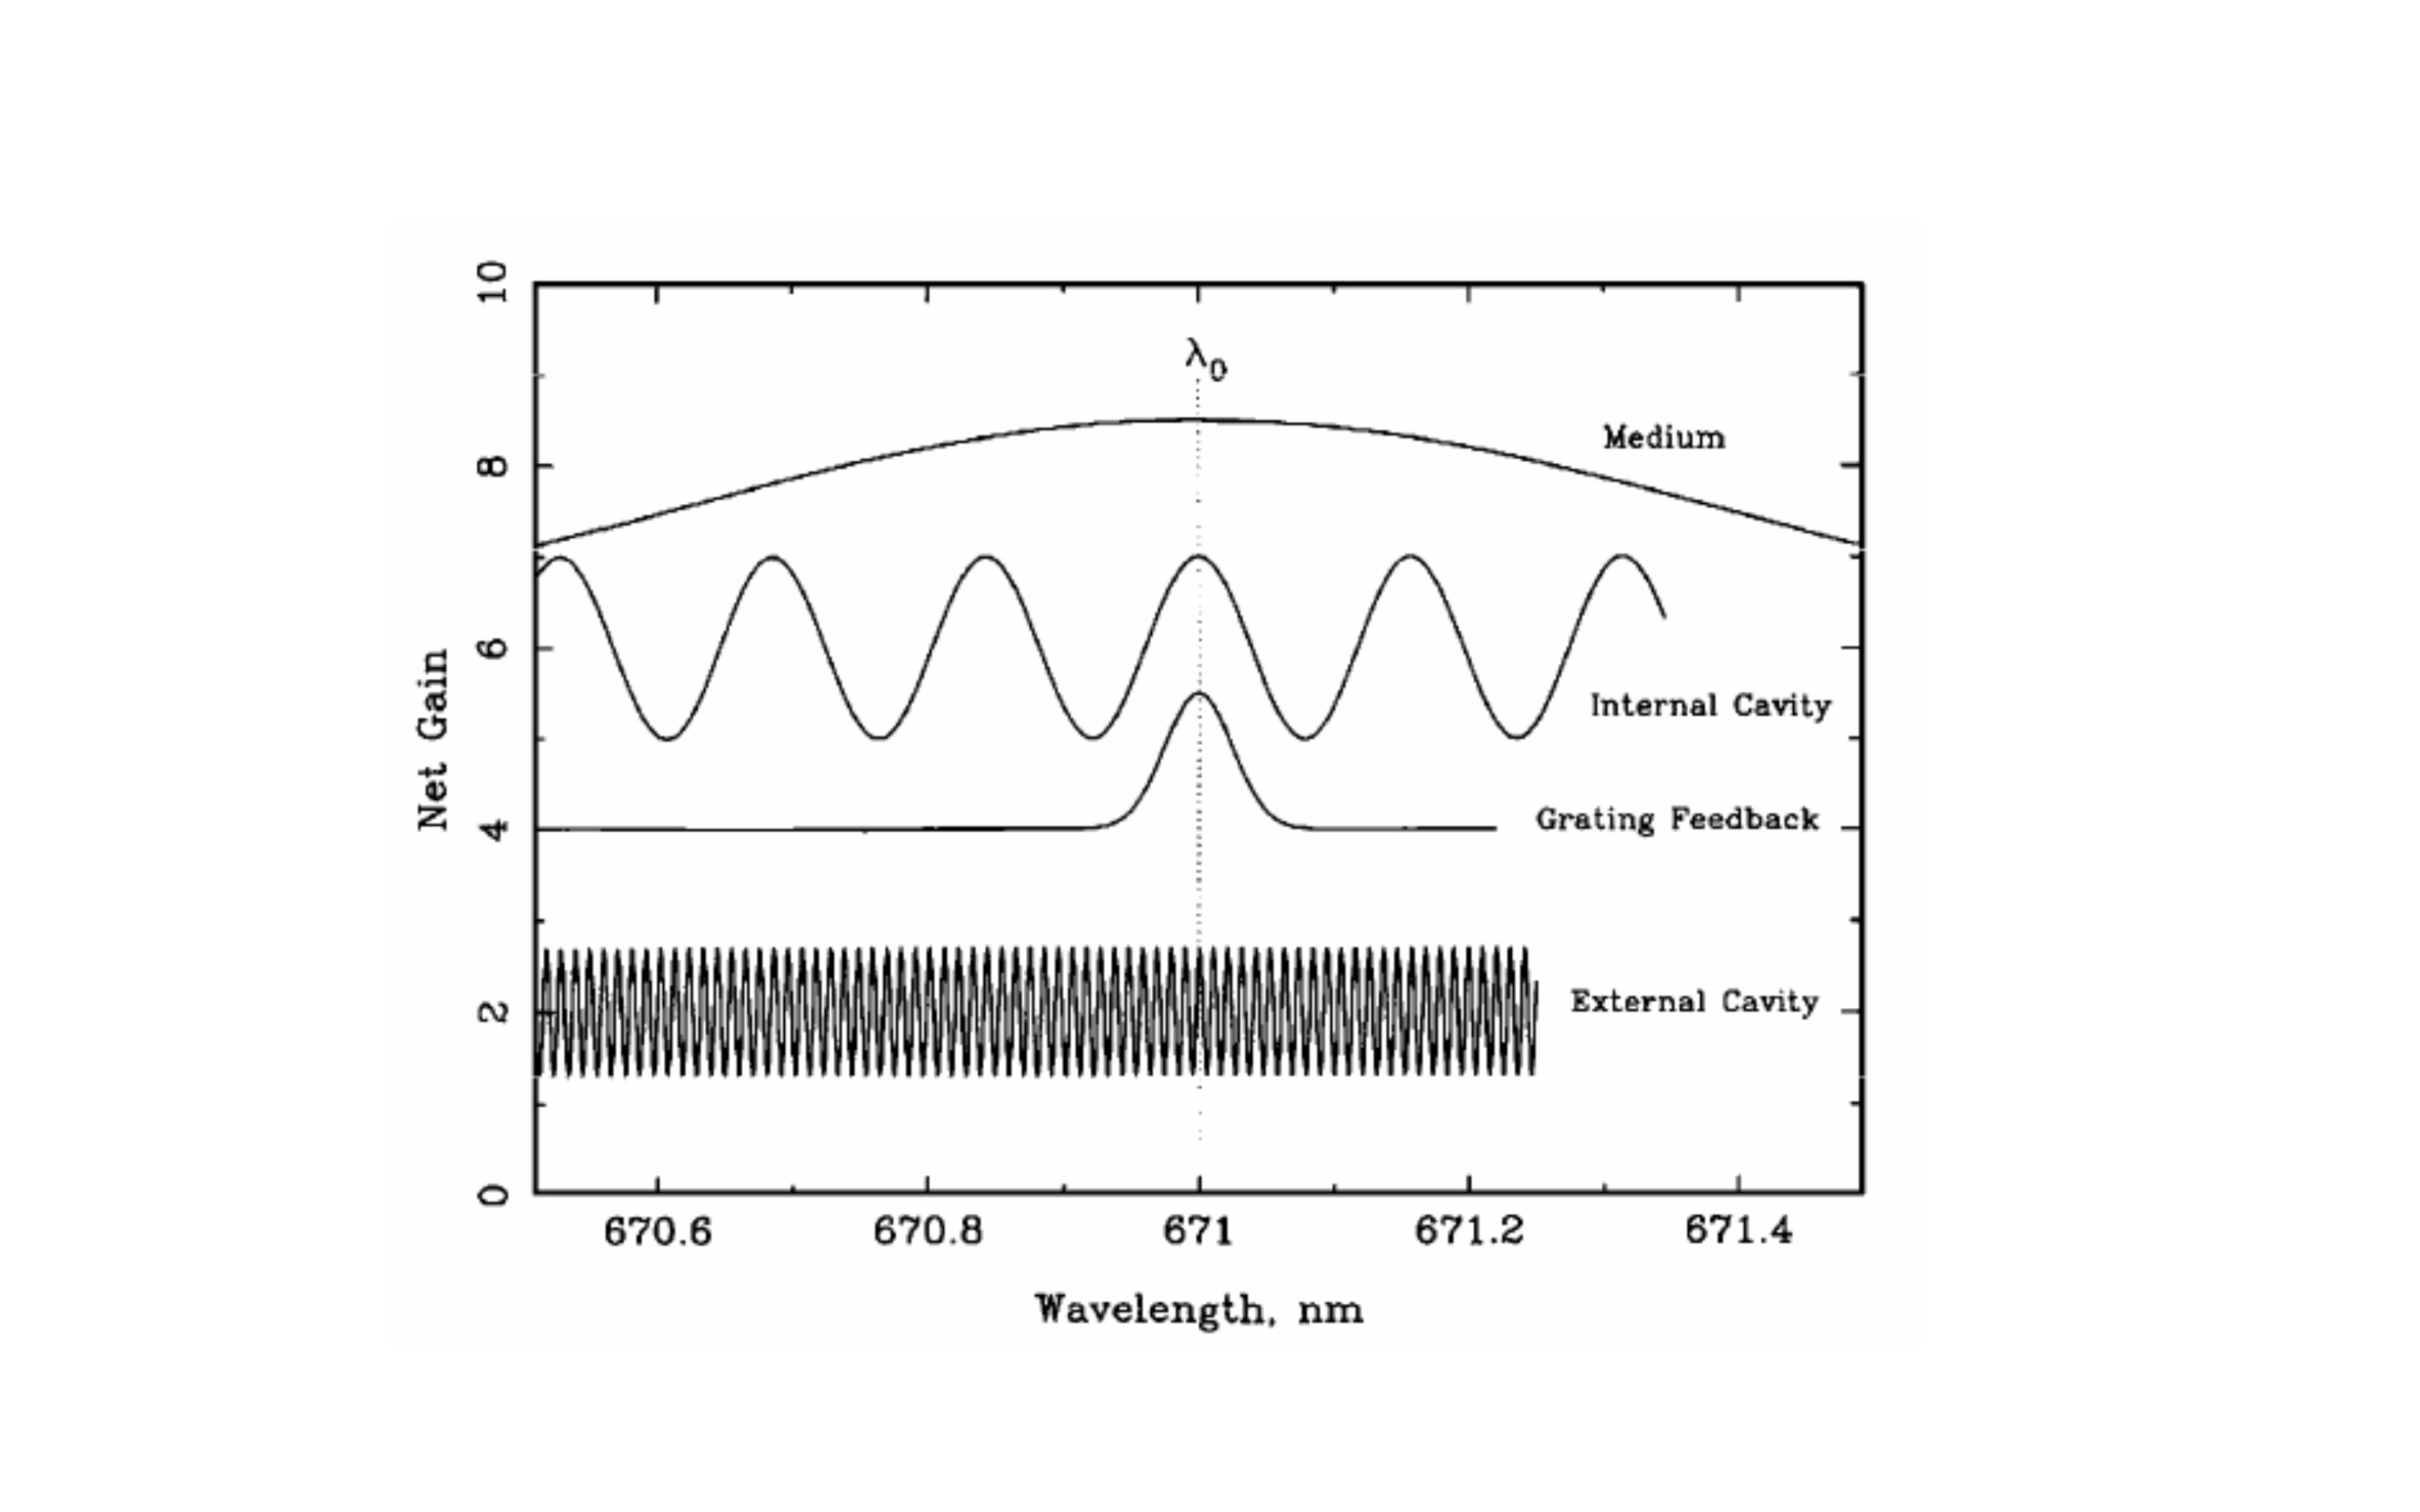
\includegraphics[width=9cm]{net_gain.pdf}
  \caption{Aufbau einer Röntgenröhre} %\cite{V603}}
  \label{fig:netgain}
\end{figure}

\begin{enumerate}
\item \textbf{Gain medium}

\noindent
A gain medium in which a population inversion is created by pumping is necessery.
In this experiment the gain medium is a semiconductor with the desired energy gap which determines the wavelength of the emitted photons.
A semiconductor is a solid material with a band gap between the positive p-doped region with an excess of holes and the negative n-doped region with an excess of electrons.
the band gap depends on the temperature as if the temperature is increased, the band gap decreases.
The net gain has its maximum at the wavelength of the emitted photons corresponding to the band gap.

\item \textbf{Internal cavity}

\noindent
The internal cavity is formed by two reflective surfaces of which only one is fully reflective.
This leads 

\item \textbf{Grating}

\noindent
The grating reflects the light in a way where the first order diffraction is sent back into the diode.
The wavelength can then be found from the bragg condition $\lambda = 2 \, d \, \text{sin}\, \theta$ where $d$ is the line spacing and $\theta$ is the grating angle.
In figure \ref{fig:netgain} the peak of the grating feedback appears at this exact wavelength, as no other wavelengths are reflected to the diode.

\item \textbf{External cavity}

\noindent


\end{enumerate}

\noindent
